\documentclass[
]{beamer}

\usepackage[english]{babel}
\usepackage[utf8]{inputenc}
\usepackage[T1]{fontenc}
\usepackage{booktabs}
\usepackage{multirow}
\usepackage{caption}
\usepackage{listings}
\usepackage{adjustbox}
%\usepackage{enumitem}
%\usepackage{setspace}
\usepackage{graphicx}

\begin{document}

	\begin{frame}
    	\frametitle{Genetic Functions}
        \begin{minipage}{0.45\textwidth}
        Initialisation
        \begin{enumerate}
            \item Random
            \item Even distribution across machines
        \end{enumerate}
        Selection
        \begin{enumerate}
            \item Fitness proportionate selection (Roulette)
            \item Stochastic universal sampling 
        \end{enumerate}
        Recombination
        \begin{enumerate}
            \item Single-Point
            \item Uniform
        \end{enumerate}
        \end{minipage}%
        \hfill
		\begin{minipage}{0.45\textwidth}
        Mutation
        \begin{enumerate}
        	\item Random Resetting
        	\item Creep Mutation
        \end{enumerate}
        Replacement (size stays)
        \begin{enumerate}
        	\item Replace-all (only Offspring)
        	\item Elitist (Best from all)
        \end{enumerate}
        \end{minipage}%
	\end{frame}
 
	\begin{frame}
    	\frametitle{Function Combinations}
        \begin{itemize}
            \item \textbf{default}\\
            Random,Roulette,Single-Point,Random,Replace-All
            \item \textbf{bad start}\\
            Random,SUS,Uniform,Creep,Elitist
           	\item \textbf{bad heuristic low variance}
            Random,Roulette,Uniform,Creep,Replace-All
            \item \textbf{good heuristic high variance}
            Even Distribution,SUS,Single-Point,Random,Elitist
            \item \textbf{good heuristic low variance}
            Even Distribution,Roulette,Uniform,Creep,Elitist
        \end{itemize}
	\end{frame}
    
	\begin{frame}
    	\frametitle{Randomized Parameter Combinations}
        
        \begin{itemize}
            \item \textbf{Parameters:} population size, mutation rate, selection rate
            \item \textbf{Without Params:} 3(Tasks)*5(Setups)*10(Iterations) = 150
           	\item \textbf{Random Search:} better coverage of the seach space
		\end{itemize}
		\vfill
        \begin{tabular}{c|c|c|c|c|c}
            \textbf{population size} & 213 & 77 & 104 & 172 & 120\\
            \textbf{selection rate} & 0.450 & 0.156 & 0.145 & 0.307 & 0.292\\
        	\textbf{mutation rate} & 0.0258 & 0.0315 & 0.0332 & 0.0083 & 0.0485
        \end{tabular}
	\end{frame}
    
    \begin{frame}
    	\frametitle{Results Task 1}
        	\begin{minipage}{\linewidth}
              \begin{table} 
              \centering
              \caption{optimal >= 6131}
                  \begin{tabular}{c|ccc|ccc}
                  {\bf name} & {\bf best} & {\bf mean} & {\bf start} & {\bf pop} & {\bf mut} & {\bf sel}\\
                  \toprule[1.pt]
                  default & {\bf 6609} & 6919 & 8136 & 77 & 0.031 & 0.156\\
                  bad start & {\bf 6160} & 6176 & 7938 & 172 & 0.008 & 0.307\\
                  bhlv & {\bf 6713} & 6774 & 8023 & 172 & 0.008 & 0.307\\
                  ghhv & {\bf 6155} & 6168 & 7114 & 172 & 0.008 & 0.307\\
                  ghlv & \textcolor{green}{\bf 6154} & 6167 & 7144 & 172 & 0.008 & 0.307\\
                  \bottomrule[1.pt]
                  \end{tabular}
              \\[10pt]
			  \caption*{Best parameter combination for each setup}
              \end{table}
        	\end{minipage}
    \end{frame}
    
    \begin{frame}
    	\frametitle{Results Task 1}
		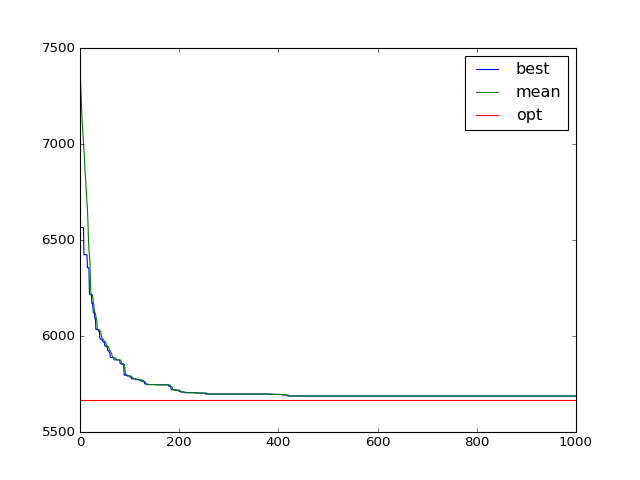
\includegraphics[width=\textwidth]{task1.png}
        \begin{center}
        it:  1000 | opt costs: 5664.671 | best: 5687.472 | mean: 5687.472
        \end{center}
    \end{frame}

    
    %%%
    \begin{frame}
    	\frametitle{Results Task 2}
        	\begin{minipage}{\linewidth}
              \begin{table} 
              \centering
              \caption{optimal >= 7959}
                  \begin{tabular}{c|ccc|ccc}
                  {\bf name} & {\bf best} & {\bf mean} & {\bf start} & {\bf pop} & {\bf mut} & {\bf sel}\\
                  \toprule[1.pt]
                  default & {\bf 8618} & 8688 & 9987 & 172 & 0.008 & 0.307\\
                  bad start & {\bf 8005} & 8024 & 10046 & 172 & 0.008 & 0.307\\
                  bhlv & {\bf 8609} & 8712 & 10085 & 172 & 0.008 & 0.307\\
                  ghhv & \textcolor{green}{\bf 8000} & 8030 & 8732 & 172 & 0.008 & 0.307\\
                  ghlv & {\bf 8008} & 8041 & 8691 & 172 & 0.008 & 0.307\\
                  \bottomrule[1.pt]
                  \end{tabular}
              \\[10pt]
			  \caption*{Best parameter combination for each setup}
              \end{table}
        	\end{minipage}
    \end{frame}
    
    \begin{frame}
    	\frametitle{Results Task 2}
		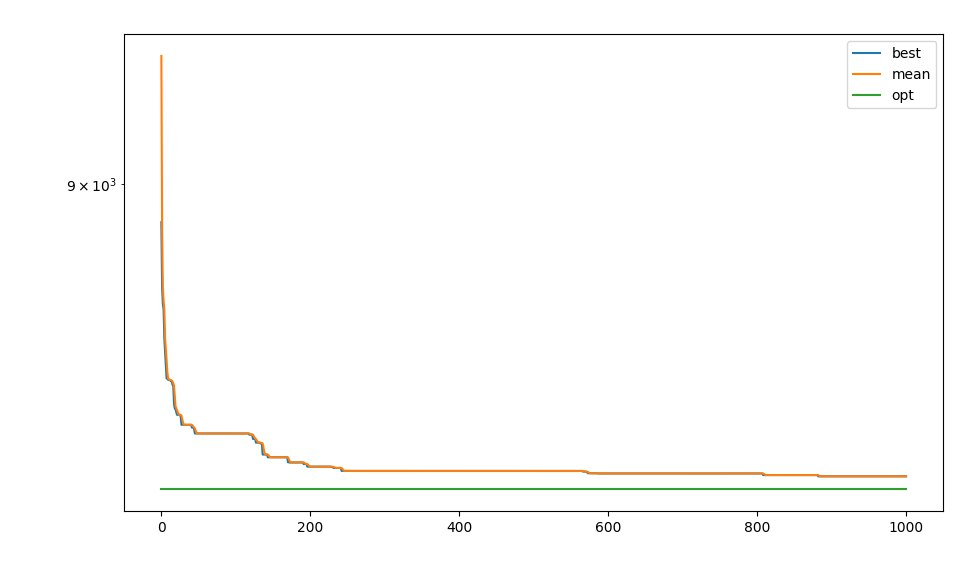
\includegraphics[width=\textwidth]{task2.jpg}
        \begin{center}
        it:  1000 | opt\_costs: 5664.671 | best: 5687.472 | mean: 5687.472
        \end{center}
    \end{frame}

    \begin{frame}
    	\frametitle{Results Task 3}
        	\begin{minipage}{\linewidth}
              \begin{table} 
              \centering
              \caption{optimal >= 150}
                  \begin{tabular}{c|ccc|ccc}
                  {\bf name} & {\bf best} & {\bf mean} & {\bf start} & {\bf pop} & {\bf mut} & {\bf sel}\\
                  \toprule[1.pt]
                  default & {\bf 223} & 228 & 304 & 77 & 0.031 & 0.156\\
                  bad start & {\bf 178} & 185 & 304 & 213 & 0.025 & 0.450\\
                  bhlv & {\bf 215} & 226 & 311 & 172 & 0.008 & 0.307\\
                  ghhv & {\bf 175} & 180 & 184 & 104 & 0.033 & 0.145\\
                  ghlv & \textcolor{green}{\bf 175} & 178 & 184 & 213 & 0.025 & 0.450\\
                  \bottomrule[1.pt]
                  \end{tabular}
              \\[10pt]
			  \caption*{Best parameter combination for each setup}
              \end{table}
        	\end{minipage}
    \end{frame} 
    
    \begin{frame}
    	\frametitle{Results Task 3}
		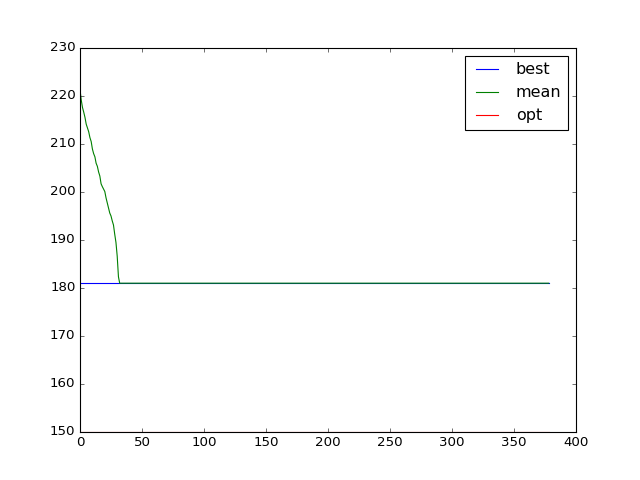
\includegraphics[width=\textwidth]{task3.png}
        \begin{center}
        it:   650 | opt costs: 150.000 | best: 181.000 | mean: 181.000
        \end{center}
    \end{frame}

    %%%
\end{document}